\subsection{Task 7: Triangle Counting}
According to the algorithms in \cite{tsourakakis2008fast}, we know that the number of triangles in a network is propotional to the sum of eigenvalue of its adjency matrix, which is $\frac{\sum_{i}\lambda_{i}^{3}}{6}$. Figure \ref{t7:timedata} shows the running time of global triangle counting with regards to the size of graph. We can see that as the size of graph increases, the running time also grows nearly linearly with the size. For the largest graph, which is Roadnet-PA, it runs nearly for an hour to complete. However, the predicted result for Roadnet-PA is unsatisfactory. We conduct both global and local triangle counting, all the data is listed as follows.

\subsubsection{Plots}
Table \ref{t7:timedata} lists run time of global triangle counting. Table \ref{t7:globalpredict} lists the predicted triangle count of each dataset. Figure \ref{t7:globaltime} plots the run time on each dataset. Figure \ref{t7:local} plots the rank-frequency plot of local triangle count on each dataset. 

\begin{table}
\begin{center}
\begin{tabular}{ | c | c | }
    \hline
    graph size & run time(seconds) \\ \hline
    7115 & 45.199s \\ \hline
    36692 & 72.76 \\ \hline
    82168 & 596.046 \\ \hline
    334863 & 1288.703 \\ \hline
    1088092 & 2980.985 \\ \hline
\end{tabular}
\end{center}
\caption{Task 7 run time(global)}
\label{t7:timedata}
\end{table}

\begin{table}
\begin{center}
\begin{tabular} {| c | c | c | c | }
    \hline
    dataset & size & predict & truth \\ \hline
    wiki-Vite & 7115 & 661282 & 608389 \\ \hline
    Enron-email & 36692 & 276757 & 727044 \\ \hline
    slash-dot & 82168 & 1294037 & 602592 \\ \hline
    Amazon-com & 334863 & 13904 & 667129 \\ \hline
    Roadnet-PA & 1088092 & 55.95 & 67150 \\ \hline
\end{tabular}
\end{center}
\caption{Predicted triangle count(global)}
\label{t7:globalpredict}
\end{table}

\begin{figure}[h]
\begin{center}
\begin{tabular}{c}
     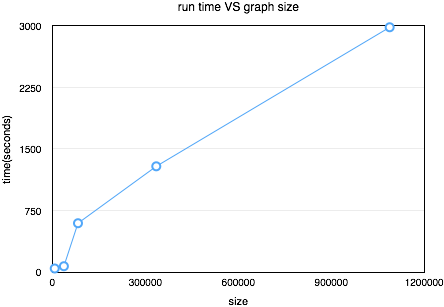
\includegraphics[width=0.8\textwidth]{FIG/t7_time.png}
\end{tabular}
\caption{Task 7: Run time VS graph size(global)}
\label{t7:globaltime}
\end{center}
\end{figure}

\begin{figure}[h]
\begin{center}
\begin{tabular}{cc}
     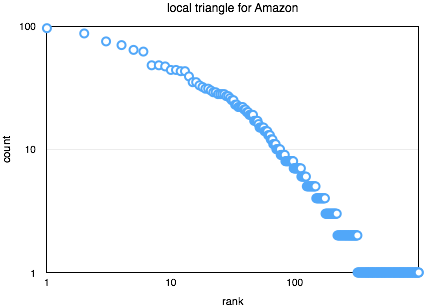
\includegraphics[width=0.4\textwidth]{FIG/t7_amazon.png} &
     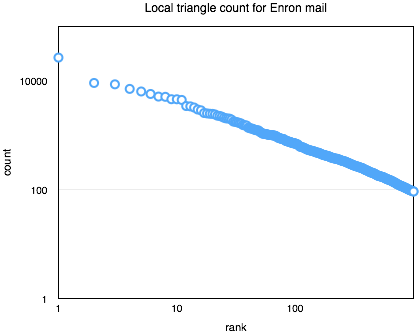
\includegraphics[width=0.4\textwidth]{FIG/t7_enron.png} \\
     (a) & (b) \\
     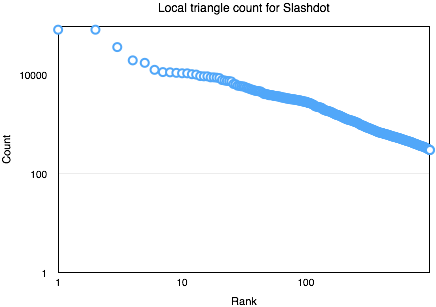
\includegraphics[width=0.4\textwidth]{FIG/t7_slashdot.png} &
     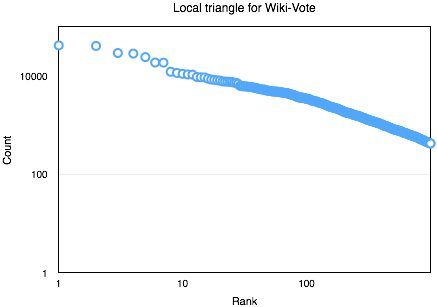
\includegraphics[width=0.4\textwidth]{FIG/t7_wikivote.png} \\
     (c) & (d) \\
     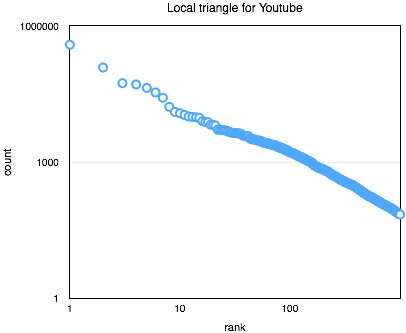
\includegraphics[width=0.4\textwidth]{FIG/t7_youtube.png} & \\
     (e)
\end{tabular}
\caption{Local triangle counting. (a) Amazon (b) Enron Mail (c) Slashdot (d) Wiki Vote (e) Youtube}
\label{t7:local}
\end{center}
\end{figure}

\subsubsection{Observation}
According to Figure \ref{t7:local}, we can see that the rank-frequency plot of local triangle count also follows power law. And we can observe that the run time grows nearly linearly with the graph size. 
